\section{Proposed PhysFormer Framework}
\label{sec:method}

\subsection{Mathematical Formulation}
Throughout this paper, we adopt the following notation: $P_{\text{load}}$, $P_{\text{pv}}$, and $P_{\text{wind}}$ denote load, PV, and wind power [MW]; $G$, $T$, and $v$ represent irradiance [W/m$^2$], temperature [$^\circ$C], and wind speed [m/s]; $\eta_{\text{pv}}$ and $\beta_T$ are the PV conversion efficiency and temperature coefficient; $v_{\text{ci}}$, $v_r$, and $v_{\text{co}}$ are the wind turbine cut-in, rated, and cut-out speeds; $a_{\text{pv}}$ and $a_{\text{wind}}$ are physics activity masks $\in[0,1]$; $g_{\text{pv}}$ and $g_{\text{wind}}$ are PGCC gates; $\alpha$ is the curriculum factor; $S=672$ and $P=96$ are the sequence and prediction lengths; and $D=512$ is the model dimension.

The forecasting target contains three VPP components: load ($P_{\text{load}}$), PV generation ($P_{\text{pv}}$), and wind generation ($P_{\text{wind}}$). Their net demand is $P_{\text{net}} = P_{\text{load}} - P_{\text{pv}} - P_{\text{wind}}$. We denote the historical component sequence by $\mathcal{X}_{\text{stat}} \in \mathbb{R}^{B \times S \times 3}$, the historical weather sequence by $\mathcal{X}_{\text{weather\_hist}} \in \mathbb{R}^{B \times S \times 3}$, and the future weather forecasts by $\mathcal{X}_{\text{weather\_future}} \in \mathbb{R}^{B \times P \times 3}$. The model outputs $Y \in \mathbb{R}^{B \times P \times 3}$, which contains the future trajectories of load, PV, and wind.

\subsection{Overall Architecture}

\begin{figure}[H]
\centering
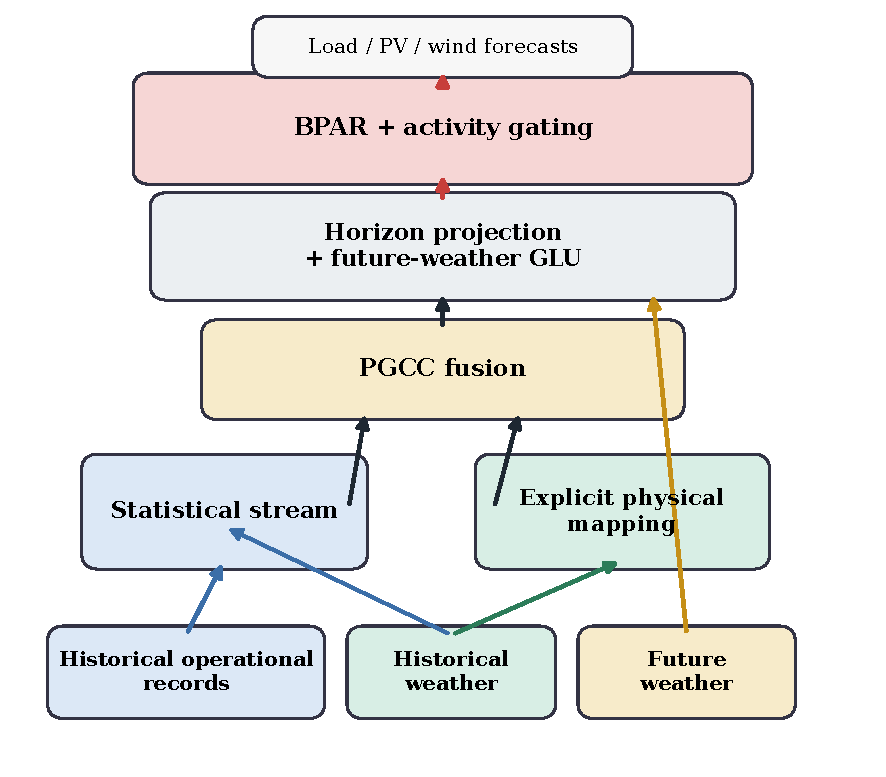
\includegraphics[width=0.98\columnwidth]{EPSR_Fig1_Architecture.pdf}
\caption{Overview of PhysFormer. Historical records and weather are processed by the statistical and explicit physical streams, fused by PGCC, conditioned on future weather, and converted into bounded component forecasts through BPAR with activity gating.}
\label{fig:overall_architecture}
\end{figure}

PhysFormer follows a compact dual-stream design. As shown in Fig.~\ref{fig:overall_architecture}, historical operational records and weather are processed by a statistical stream and an explicit physical stream. The two branches are fused in PGCC, conditioned on future weather through a gated linear unit (GLU), and mapped to bounded component forecasts by BPAR with activity gating. The statistical stream uses a Transformer encoder ($d_{\text{model}}=512$, $d_{\text{ff}}=1024$, $8$ heads, $3$ layers). The physical stream produces theory-based baselines from weather variables before fusion.

\subsection{Explicit Physical Mapping}
The explicit physical mapping layer injects physics by mapping weather variables to theory-based power baselines.

\subsubsection{PV Model}
The theoretical PV generation is driven by irradiance $G$ and degraded by cell temperature, modeled as:
\begin{equation}
    P_{\text{pv}} = G \cdot \eta_{\text{pv}} \cdot \text{clamp}(1 - \beta_T \cdot (T - 25), 0, 1.5)
\label{eq:pv_model}
\end{equation}
where $T$ is the temperature. The learnable conversion efficiency is $\eta_{\text{pv}} = 0.33 \cdot \sigma(\theta_{\text{eff}})$, and the temperature coefficient is $\beta_T = \text{softplus}(\theta_{\text{temp\_coef}}) \times 0.01 \in [0.003, 0.005]/^\circ\text{C}$.

\subsubsection{Wind Model}
Wind power is largely determined by three operating thresholds: the cut-in speed $v_{\text{ci}}$, rated speed $v_{\text{r}}$, and cut-out speed $v_{\text{co}}$. To preserve their order during training, we use a cumulative delta form: $v_{\text{ci}} = \text{softplus}(\theta_{\text{ci}})$, $v_{\text{r}} = v_{\text{ci}} + \text{softplus}(\theta_{\text{r\_delta}})$, and $v_{\text{co}} = v_{\text{r}} + \text{softplus}(\theta_{\text{co\_delta}})$. The power output then follows an idealized soft curve:
\begin{equation}
    P_{\text{wind}} = \text{scale}_{\text{wind}} \cdot \sigma(5 \cdot (w_{\text{norm}} - 0.5)) \cdot I_{\text{running}}
\label{eq:wind_ideal}
\end{equation}
where $w_{\text{norm}}$ is the normalized speed, $scale_{\text{wind}}$ is a learnable amplitude factor, and $I_{\text{running}}$ is 1 within $[v_{\text{ci}}, v_{\text{co}}]$ and 0 otherwise. To maintain differentiability, PhysFormer replaces $I_{\text{running}}$ with a continuous physics activity mask $a_{\text{wind}}$ (detailed in Section~\ref{subsec:activity_gating}):
\begin{equation}
    P_{\text{wind,actual}} = \text{scale}_{\text{wind}} \cdot \sigma(5 \cdot (w_{\text{norm}} - 0.5)) \cdot a_{\text{wind}}
\label{eq:wind_actual}
\end{equation}
This design keeps the threshold structure differentiable and avoids Straight-Through Estimators. The cumulative delta form also preserves the ordering of the operating limits during training.

\subsubsection{Load Model}
We abstract the power load variations triggered by human cooling and heating activities through a quadratic thermal comfort model:
\begin{equation}
    P_{\text{load}} = P_{\text{base}} + \text{softplus}(\gamma) \cdot (T - T_c)^2
\label{eq:load_model}
\end{equation}
where $T_c$ is an optimizable thermal comfort baseline initialized at $20^\circ\text{C}$. In our design, the Transformer captures the main temporal patterns of load, while the physical mapping stream captures the temperature-driven deviation around that baseline.

\noindent
Fig.~\ref{fig:physical_mapping} shows the mappings that determine the physical activation boundaries most directly. We visualize PV and wind because boundary handling is most critical in these channels. The learned load comfort parameters are reported in Table~\ref{tab:physical_params}.

\begin{figure}[H]
\centering

\includegraphics[width=0.98\columnwidth]{EPSR_Fig2_PhysicalMapping.pdf}
\caption{The learned PV and wind mappings preserve physically meaningful monotonicity and operating thresholds. The PV branch maintains smooth temperature degradation, while the wind branch retains the cut-in, rated, and cut-out structure reported in Table~\ref{tab:physical_params}.}
\label{fig:physical_mapping}
\end{figure}

\subsubsection{Physics Activity Gating}
\label{subsec:activity_gating}
To reduce non-physical artifacts, we introduce an explicit activity gate. For PV, $a_{\text{pv}} = \tanh(10 \cdot P_{\text{pv\_theory}})$. For wind, $a_{\text{wind}} = \tanh(10 \cdot \text{softplus}(v - v_{\text{ci}}) \cdot \text{softplus}(v_{\text{co}} - v))$. The load uses $a_{\text{load}} = 1$. These masks keep the model differentiable and connect active operating states to null-generation periods.

\subsection{Physics-Guided Gating and Alignment (PGCC)}
The Physics-Guided Gating and Alignment (PGCC) module coordinates the interaction between the statistical stream and the physically encoded representations. In this work, PGCC guides weather-response behavior and improves alignment with known physical cues. It is not intended to infer causality from data alone.

\subsubsection{Physics-Anchored Illumination Prior}
We first build an illumination prior to suppress spurious activation. The prior is defined as $p_{\text{pv}}^{\text{prior}} = \sigma(k_{\text{irr}} \cdot (G_{\text{norm}} - \theta_{\text{irr}}))$, with $\theta_{\text{irr}} \in [-2.0, 0.5]$ and slope $k_{\text{irr}} \in [1, 100]$. This term separates day from night and reduces the impact of noisy activations in the data embeddings.

\subsubsection{Volatility-Aware Soft Gate}
To adapt the trust placed in the physical stream, we compute a sequence-level volatility term $\upsilon = \frac{1}{C}\sum_{c}\text{Var}_{t}(\mathcal{X}_{\text{weather},c})$. This term, together with the statistical embeddings and attention outputs, is fed to a downsampling multilayer perceptron that produces the soft gate maps.

\subsubsection{Source-Differentiated Gate Bounds}
The coupling implements separate activation ranges to accommodate generation source characteristics:
\begin{gather}
    \text{gate}_{\text{pv}} = \text{smooth} \left( p_{\text{pv}}^{\text{prior}} \cdot (0.5 + g_{\text{soft\_pv}}) \right) \in [0, 1.5] \label{eq:gate_pv} \\
    \text{gate}_{\text{load}} = \text{smooth}(g_{\text{soft\_load}}) \in [0, 1.0] \label{eq:gate_load}
\end{gather}
The upper bound of $1.5$ for $\text{gate}_{\text{pv}}$ leaves headroom for the residual stream. This is useful during transient conditions such as short over-irradiance events. With gate-response regularization, the learned $\text{gate}_{\text{pv}}$ reaches a Pearson correlation of $r=0.8306$ with irradiance. Fig.~\ref{fig:gate_alignment} shows this alignment.

\subsubsection{Physics-to-Data Curriculum Transition}
We condition the alignment phase via a curriculum factor $\alpha$. As the fusion queries retrieve features, the module integrates inputs dynamically scaled as:
\begin{equation}
    q = \alpha \cdot F_{\text{physics}} + (1 - \alpha) \cdot g_{\text{soft}} \cdot F_{\text{stat}}
\label{eq:curriculum_query}
\end{equation}
At the start of training ($\alpha \to 1$), the queries rely more on the physical representations. As training proceeds ($\alpha \to 0$), the model gradually shifts toward the data-driven residual states gated by $g_{\text{soft}}$.

\subsubsection{Temporal Smoothing}
Raw gate values can be locally discontinuous. We therefore smooth all temporal gating variables with a grouped one-dimensional depthwise convolution (kernel size $3$, groups=$d_{\text{model}}$).

\subsection{Exogenous Weather Integration}
After horizon projection, the model incorporates future weather information that is not available in the history sequence alone. We concatenate the future physical latent space $F_{\text{weather\_future}}$ with the history representation $F_{\text{history}}$ and fuse them with a Gated Linear Unit:
\begin{equation}
    F_{\text{future}} = \text{gate} \cdot \text{proj}(F_{\text{cat}}) + F_{\text{history}}
\end{equation}
This step conditions the residual heads on upcoming weather changes such as dawn transitions or wind cut-outs.

\subsection{Bounded Physical Act-Residual (BPAR) Mechanism} \label{subsec:bpar}
To reduce non-physical anomalies while preserving gradient flow, we propose the Bounded Physical Act-Residual (BPAR) mechanism. Let $\mu_x$ and $\sigma_x$ denote the global mean and standard deviation of component $x$. We define the normalized physical zero-point as $P_{x,\text{zero}} = (0 - \mu_x) / \sigma_x$. BPAR combines the theory baseline with the neural residual through a differentiable Softplus form:
\begin{equation}
    \hat{P}_{x,\text{raw}} = \text{Softplus}\Big((P_{x,\text{theory}} + r_x) - P_{x,\text{zero}}\Big) + P_{x,\text{zero}}
\label{eq:bpar}
\end{equation}
Because $\text{Softplus}(z) > 0$ for all $z$, this form keeps $\hat{P}_{x,\text{raw}} > P_{x,\text{zero}}$ in the normalized domain. Under the adopted normalization and anti-normalization setting, the output remains structurally non-negative for $\sigma_x > 0$. We further use a small numerical floor $\epsilon=10^{-5}$ for degenerate variance cases such as night-time PV.

The prediction is then fused with the physics activity mask $a_x \in [0, 1]$:
\begin{equation}
    \hat{P}_{x,\text{final}} = a_x \cdot \hat{P}_{x,\text{raw}} + (1 - a_x) \cdot P_{x,\text{zero}}
\label{eq:activity_mask}
\end{equation}
When $a_x \to 0$, BPAR smoothly pulls the output toward the physical zero baseline. Compared with unconstrained predictors, it reduces boundary violations at the cost of small local corrections near the boundary.

\noindent
Because the main benefit of BPAR appears near the zero boundary, Fig.~\ref{fig:bpar_mechanism} visualizes the output manifold and the role of activity gating around shutdown transitions.

\begin{figure}[!htbp]
\centering
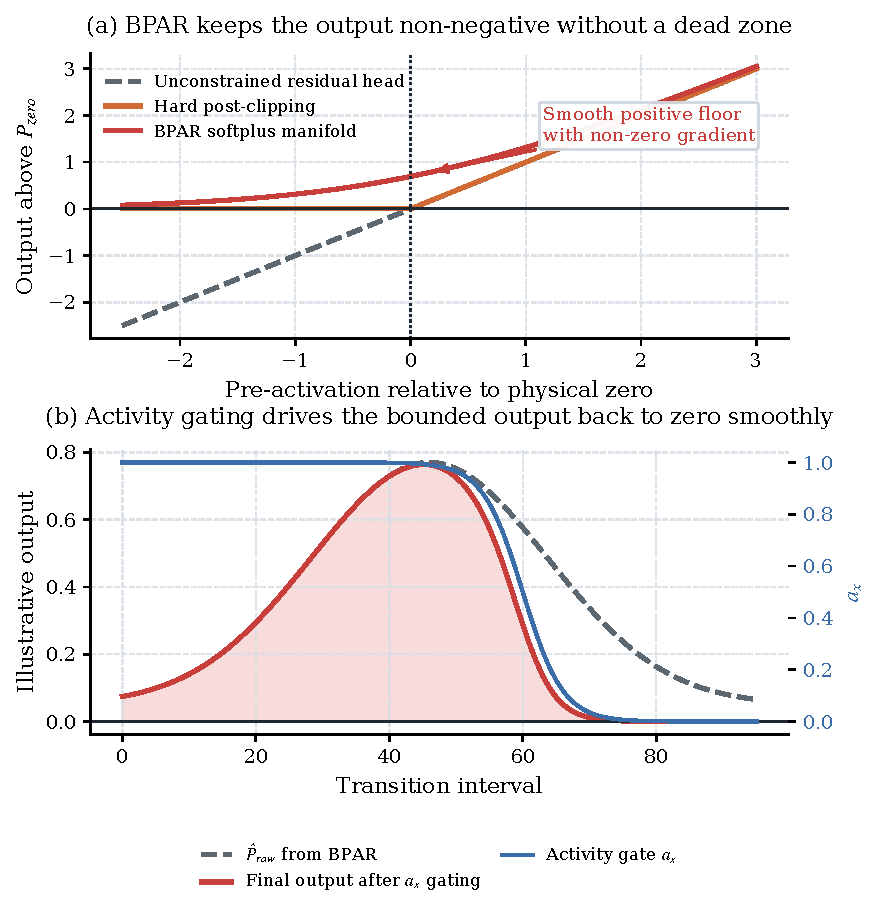
\includegraphics[width=0.92\columnwidth]{EPSR_Fig3_BPARMechanism.pdf}
\caption{BPAR removes the hard dead zone of post-clipping and, together with activity gating, smoothly pulls the forecast back toward the physical zero boundary. Panel (b) is an illustrative mechanism plot under the adopted normalization setting.}
\label{fig:bpar_mechanism}
\end{figure}

\begin{figure}[tbp]
\centering

\includegraphics[width=0.94\columnwidth]{EPSR_Fig4_GateAlignment.pdf}
\caption{PGCC keeps the learned PV gate aligned with irradiance over both representative windows and the saved visualization subset. The full-test Pearson correlation reported in the text remains $r=0.8306$.}
\label{fig:gate_alignment}
\end{figure}

\FloatBarrier

\subsection{Physics-Constrained Curriculum Training}
\label{subsec:training}

Training with physical constraints introduces conflicts between the forecasting loss and the physics losses. We therefore use a Physics-Constrained Curriculum Training strategy. It separates metric spaces, balances amplitudes dynamically, and activates constraints in phases.

\subsubsection{Loss Function Design}
The regression loss (MSE) is computed in normalized space for stable optimization. All physics constraints ($L_{\text{phys}}$) are computed after denormalization in MW. We use six penalties (Table~\ref{tab:losses}): four soft constraints for structure and two hard constraints for safety-critical violations.

\begin{table}[htbp]
\caption{Components of Physics-Guided Loss Function}
\label{tab:losses}
\centering
\footnotesize
\setlength{\tabcolsep}{3pt}
\begin{tabularx}{\columnwidth}{@{}llc>{\raggedright\arraybackslash}X@{}}
\toprule
\textbf{Comp.} & \textbf{Wt.} & \textbf{Formula} & \textbf{Motivation} \\ \midrule
$L_{\text{net}}$ (Soft) & 1.0 & $|\sum \hat{y}_{\text{comp}} - y_{\text{net}}|$ & Ensures models sum to net demand. \\
$L_{\text{energy}}$ (Soft) & 0.5 & $|\mathbb{E}_t[\hat{y}] - \mathbb{E}_t[y]|$ & Enforces macro energy conservation. \\
$L_{\text{deriv}}$ (Soft) & 0.3 & $|\Delta \hat{y} - \Delta y|$ & Captures ramp rate magnitudes. \\
$L_{\text{dir}}$ (Soft) & 0.1 & $\mathbb{E} [1 {-} \text{sim}_{\text{cos}}]$ & Preserves accurate trend switching. \\ \midrule
$L_{\text{bvr}}$ (Hard) & 2.0 & $\mathbb{E} [(\max(0, -\hat{y}_{\text{real}}))^2]$ & Penalizes negative power strictly. \\
$L_{\text{rvr}}$ (Hard) & 2.0 & $\mathbb{E} [(\max(0, |\Delta\hat{y}| {-} \rho_k))^2]$ & Penalizes sudden jumps. \\ \bottomrule
\end{tabularx}
\end{table}

We use an adaptive amplitude balancing factor $\gamma_{\text{ema}}$ to track the ratio between forecast error and physical loss:
\begin{equation}
    \gamma_{\text{ema}} \leftarrow 0.9 \cdot \gamma_{\text{ema}} + 0.1 \cdot \left( \frac{L_{\text{mae\_phys}}}{L_{\text{phys\_ref}}} \right)
\label{eq:gamma_ema}
\end{equation}
where $L_{\text{phys\_ref}}$ is the total unweighted physical loss in MW. This term yields a dimensionless multiplier. It is set to $1.0$ for the first 50 batches, frozen when curriculum activation is below $0.05$, and clamped to $[0.1, 10.0]$. The combined objective becomes:
\begin{equation}
    L_{\text{total}} = L_{\text{mse}}(\text{normalized}) + \gamma_{\text{ema}} \cdot L_{\text{phys\_weighted}}(\text{MW})
\label{eq:total_loss}
\end{equation}

Note: while BPAR provides a structural output floor, $L_{\text{bvr}}$ remains essential during training to provide gradient signals that prevent latent representations from drifting into non-physical regimes.

\subsubsection{Four-Phase Curriculum}
To stabilize optimization, we use the four-phase constraint schedule listed in Table~\ref{tab:curriculum}.

\begin{table}[htbp]
\caption{Four-Phase Physics Curriculum and Layer-wise Learning Rates}
\label{tab:curriculum}
\centering
\scriptsize
\setlength{\tabcolsep}{2pt}
\begin{tabularx}{\columnwidth}{@{}lc>{\raggedright\arraybackslash}p{1.8cm}>{\raggedright\arraybackslash}X@{}}
\toprule
\textbf{Phase} & \textbf{Ep.} & \textbf{Active Const.} & \textbf{Notes} \\ \midrule
I (Init.) & 0--4 & None & Physics frozen; base mapping. \\
II (Safety) & 5--14 & $L_{\text{net}}, L_{\text{bvr}}$, $L_{\text{rvr}}, L_{\text{dir}}$ & Safety bounds ramped. \\
III (Integ.) & 15--29 & Phase II + $L_{\text{energy}}, L_{\text{deriv}}$ & Macro conservation. \\
IV (Satur.) & 30--99 & All & Full regularized training. \\ \midrule
\multicolumn{4}{@{}l}{\textbf{Layer-wise Learning Rates}} \\ \midrule
\multicolumn{2}{@{}l}{Physics (ExplicitPhysicalMapping)} & $10^{-5}$ & Preserves priors. \\
\multicolumn{2}{@{}l}{Gating (PGCC)} & $5{\times}10^{-5}$ & Stable alignment. \\
\multicolumn{2}{@{}l}{Statistical (all other)} & $10^{-4}$ & Fast convergence. \\
\bottomrule
\end{tabularx}
\end{table}

The curriculum introduces the constraints progressively. Phase I learns the statistical backbone with frozen physics parameters. Phase II focuses on safety boundaries. Phase III adds macro-level structure. Phase IV activates the full objective. Each constraint weight is ramped with a bounded sigmoid. The PGCC alignment coefficient follows $\alpha = 1.0 - w_{\text{curr\_net}}$.

\subsubsection{Layer-wise Learning Rates}
We further separate the optimizer into three AdamW parameter groups (Table~\ref{tab:curriculum}, bottom). The statistical backbone uses a learning rate of $1 \times 10^{-4}$. After epoch 5, the physical parameters are unfrozen at $1 \times 10^{-5}$, and the PGCC parameters use $5 \times 10^{-5}$.

\subsubsection{Regularization and Early Stopping}
We use three regularization paths. First, a Physics Prior Regularizer compares the learned physical parameters with nameplate values by mean squared error (weight 0.1). Second, a Gate Response Regularization anchors the temporal PV gate to irradiance (weight 0.05), with dynamic masking when the prior variance $\sigma^2_{\text{prior}} < 10^{-3}$ to avoid night-time noise.

\textbf{Role of PGCC:} In this framework, PGCC mainly improves gate alignment and interpretability rather than raw forecasting accuracy. The final prediction is still produced by the residual pathway, so the alignment term can shape weather-response behavior without dominating the forecasting loss.

Gradient clipping uses a dynamic bound of $0.5$ during critical curriculum transitions ($0.1 < w_{\text{curr\_net}} < 0.9$), releasing to $1.0$ otherwise. Early stopping uses channel-equalizing $NRMSE_{\text{avg}}$ with patience of 15 epochs.
